\documentclass[UTF8]{ctexart}
\usepackage{setspace}
\usepackage[letterpaper,top=2cm,bottom=2cm,left=3cm,right=3cm,marginparwidth=1.75cm]{geometry}
\CTEXsetup[format={\Large\bfseries}]{section}
\usepackage{amsmath}
\usepackage{mathabx}
\usepackage[mathscr]{eucal}
\usepackage{graphicx}
\title{Numerical Analysis HW4}
\author{数学与应用数学2002 王锦宸 }
\date{November 2022}

\begin{document}

\maketitle
\section{}
 The normalized FPN of 477 is $1.11011101 \times 2^8$.
\section{}
 The normalized FPN of $\frac{3}{5}$ is $1.001\;1001\dots \times 2^{-1}$.
\section{}
 Let the normalized representation of $x = 1.000\dots0 \times \beta ^e$(there are p digits).\\
Thus, $x_L = \overline{(\beta -1).(\beta-1)(\beta-1)\dots(\beta-1)0} \times \beta ^{e-1}$, $x_R = 1.000\dots1 \times \beta^e$.\\
Then, we have $x_R - x = \beta ^{e-p}$ and $x - x_L = \beta ^{e-p-1}$, therefore $x_R - x = \beta(x-x_L)$.
\section{}
 $x_L = 1.001\; 1001\; 1001\; 1001\; 1001\; 1001 \times 2^{-1}$, $x_R = 1.001\;1001\;1001\;1001\;1001\;1010 \times 2^{-1}$
Thus, $x-x_L = \frac{3}{5} \times 2^{-24}$, $x_R - x = \frac{2}{5} \times 2^{-24}$,$fl(x) = x_R$ and $error\;=\frac{2}{3} \times 2^{-24}$
\section{}
 It'll be $\epsilon = 2 ^{-23}$
\section{}
 \noindent $fl(cos(\frac{1}{4})) = (0.1111100\dots) \times 2^{0} =(1.1111100\dots) \times 2^{-1}$, \\$fl(1) = (1.0000\dots0 )\times 2^0$.\\
Thus, $fl(1) - fl(cos(\frac{1}{4})) = (0.0000011\dots) \times 2^0 = (1.1\dots) \times 2^{-6}$\\
It loses 6 bits of precision.
\section{}
 \noindent 1.Taylor Expansion   1 - cos(x) = $1 - (1-\frac{x^2}{2!}+\frac{x^4}{4!}-\dots) = \frac{x^2}{2!}-\frac{x^4}{4!}+\dots$\\
2.Use trigonometric formula   $1 - cos(x) = 2sin(\frac{x}{2})^2$
\section{}
\noindent  · $f(x) = (x-1)^\alpha , f'(x) = \alpha(x-1)^{\alpha - 1},C_f(x) = |\frac{\alpha x(x-1)^{\alpha - 1}}{(x-1)^{\alpha}}| = \alpha \frac{x}{x-1}$. Thus, when $\alpha \neq 0$, $C_f(x)$ is large when $x \rightarrow \infty$\\
· $f(x)=\ln (x), f'(x) = \frac{1}{x}, C_{f}(x)=\left|\frac{1}{\ln (x)}\right|, C_{f}(x)$is large when  $x \rightarrow 0 .$\\
· $ f(x)=e^{x}, f'(x) = e^{x}, C_{f}(x)=|x|, C_{f}(x)$ is large when  $|x| \rightarrow \infty .$\\
· $f(x)=\arccos (x), C_{f}(x)=\left|\frac{x}{\sqrt{1-x^{2}} \arccos (x)}\right|, C_{f}(x)$  is large when  $|x| \rightarrow 1 .$
\section{}
\subsection{}
$f(x) = 1 - e^{-x}$, $f'(x) = e^{-x}$, $C_f(x) = |\frac{x}{e^x-1}|$\\
It's monotonically descending in [0,1] and $C_f(x)_{max} = C_f(0) = 1$, thus $C_f(x) \in [0,1]$.
\subsection{}
$\operatorname{cond}_{A}(x)=\frac{1}{\epsilon_{u}} \inf _{f\left(x_{A}\right)=f_{A}(x)} \frac{\left|x_{A}-x\right|}{|x|} . \text { Because }\; \forall x \in \mathbf{F},\left|f(x)-f_{A}(x)\right|=\left|f(x)-f\left(x_{A}\right)\right|=\left|f^{\prime}(\xi)\right| \mid x-x_{A} \mid \leq e \epsilon_{u}, \xi \in\left[x, x_{A}\right] \text {, so }\; \operatorname{cond}_{A}(x) \leq \frac{e}{|x|} .$

\subsection{}
\noindent The following graph depicts $cond_f$ and the upper bound $cond_A$ on $[0,1]$.
\begin{figure}[htp]
    \centering
    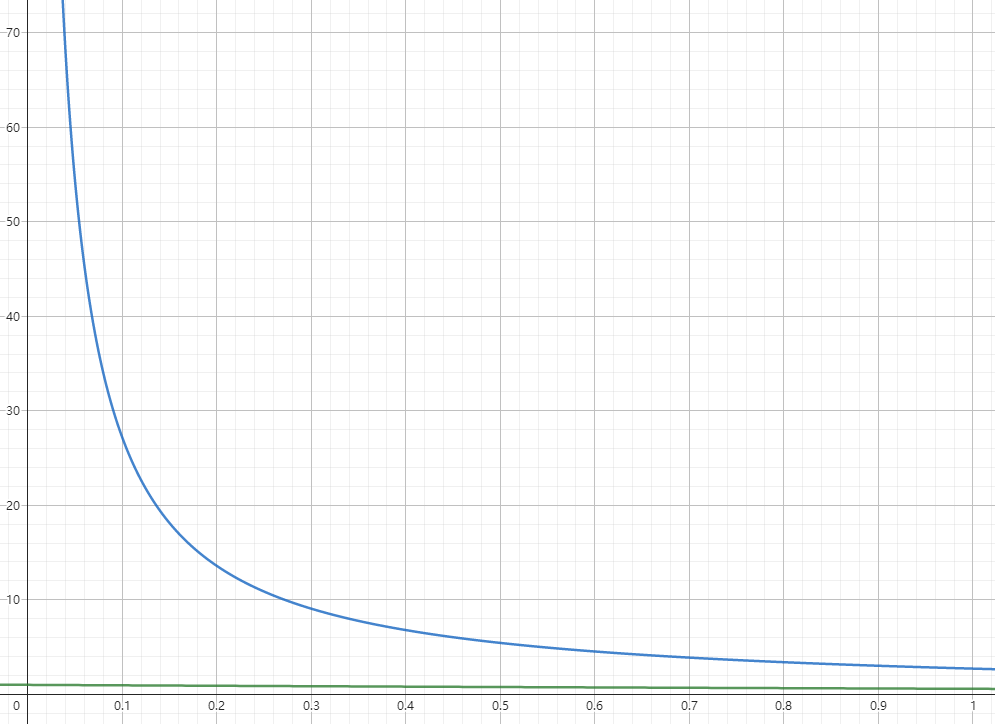
\includegraphics[width=10cm]{plot.png}
    \caption{$cond_f$ and $cond_A$}
    \label{fig:1L}
\end{figure}

\noindent From the graph, we know that $cond_f$ is small on the whole interval while $cond_A \rightarrow \infty \text{ when } x \rightarrow 0$\\
We notice that f(0) = 0 and $f_{A}(x)=f(x)(1+\delta(x))$. When $\delta (x) \rightarrow \infty , $

\section{}
For $r=f\left(a_{0}, a_{1}, \cdots, a_{n-1}\right) \neq 0, a_{i}(x)=\left|\frac{a_{i} \frac{\partial r}{\partial a_{i}}}{r}\right| .$ Since  r  is the root of  p(x), $\sum_{i=0}^{n-1} a_{i} r^{i}=0$ , we have  $\frac{\partial r}{\partial a_{i}}=-\frac{r^{i}}{\sum_{j=1}^{n-1} j a_{j} r^{j-1}}=-\frac{r^{i}}{p^{\prime}(r)} \cdot a_{i}(x)=\left|\frac{a_{i} r^{i-1}}{p^{\prime}(r)}\right| .$Thus
$\operatorname{cond}_{f}(x)=\|A(x)\|_{1}=\max _{i} a_{i}(x)=\max _{i}\left|\frac{a_{i} r^{i-1}}{p^{\prime}(r)}\right| .$\\
\indent  Put it into Wilkinson example, consider the condition number for  $f(x)=\prod_{k=1}^{p}(x-k)$ , at point  p , we have $\operatorname{cond}_{f}(x)=\max _{i}\left|\frac{a_{i} p^{i-1}}{(p-1) !}\right| \geq \frac{\sum_{k=1}^{p} k p^{p-2}}{(p-1) !}=\frac{(p+1) p^{p-1}}{2(p-1) !} $. Thus we know that the difficulty of solving polynomials with high degrees is out of its high condition number.

\section{}
In the FPN system (2,2,-1,1), $a = 1.0 \times 2^0$, $b = 1.1 \times 2^0$. Then $\frac{a}{b} = 0.101 $(of precision 4), so $fl(\frac{a}{b}) = 1.0 \times 2^{-1}$ and $error(\frac{a}{b}) = 0.01 = \epsilon_u$, which is contradictory to the model of arithmetic.

\section{}
In IEEE 754, the parameters of single precision FPN is (2,24,-126,127). The root in the interval $[128,129]$ will be represented as $m \times 2^7$, thus the distance between adjacent floating point is $2^7 \times \epsilon_M = 2^{-16} \approx 1.525 \times 10^{-5} > 10 ^{-6}.$

\section{}
$\text { For } s(x)=a x^{3}+b x^{2}+c x+d$, we need to know the values of $s(x), s'(x)$ at $x_i, x{i+1}$.Thus we need to solve the equations with the coefficient matrix,
\begin{equation}
    \left[\begin{array}{cccc}
x_{i}^{3} & x_{i}^{2} & x_{i} & 1 \\
x_{i+1}^{3} & x_{i+1}^{2} & x_{i+1} & 1 \\
3 x_{i}^{2} & 2 x_{i} & 1 & 0 \\
3 x_{i+1}^{2} & 2 x_{i+1} & 1 & 0
\end{array}\right]\left[\begin{array}{l}
a \\
b \\
c \\
d
\end{array}\right]=\left[\begin{array}{c}
f\left(x_{i}\right) \\
f\left(x_{i+1}\right) \\
f^{\prime}\left(x_{i}\right) \\
f^{\prime}\left(x_{i+1}\right)
\nonumber
\end{array}\right]
\end{equation}
 When $x_i$ is close to $x_{i+1}$, the condition number will be large, thus it will get inaccurate number.

 \section*{Programming 1}
 The output of 10 equally spaced points between [0.99, 1.01] is,(It's just for display and we draw the plot with 100 points )
 \begin{equation}
    \begin{array}{|c|c|c|}
        \hline \mathrm{f} & \mathrm{g} & \mathrm{h} \\
         \hline1.77636e-15 &-1.11022e-15 &1e-16\\
        \hline3.55271e-15 &-6.66134e-16 &1.67772e-17\\
        \hline5.32907e-15& 9.99201e-16 &1.67962e-18\\
        \hline0 &-3.55271e-15& 6.5536e-20\\
        \hline1.77636e-15& 1.0103e-14 &2.56e-22\\
        \hline0 &0 &0\\
        \hline-1.24345e-14 &2.22045e-16& 2.56e-22\\
        \hline3.55271e-15& -1.77636e-15& 6.5536e-20\\
        \hline5.32907e-15& -2.44249e-15 &1.67962e-18\\
        \hline-3.55271e-15&2.66454e-15& 1.67772e-17\\
        \hline1.95399e-14 &8.88178e-16& 1e-16\\
        \hline
    \nonumber
    \end{array}
 \end{equation}
 and the figure is,\\
 \begin{figure}[htp]
    \centering
    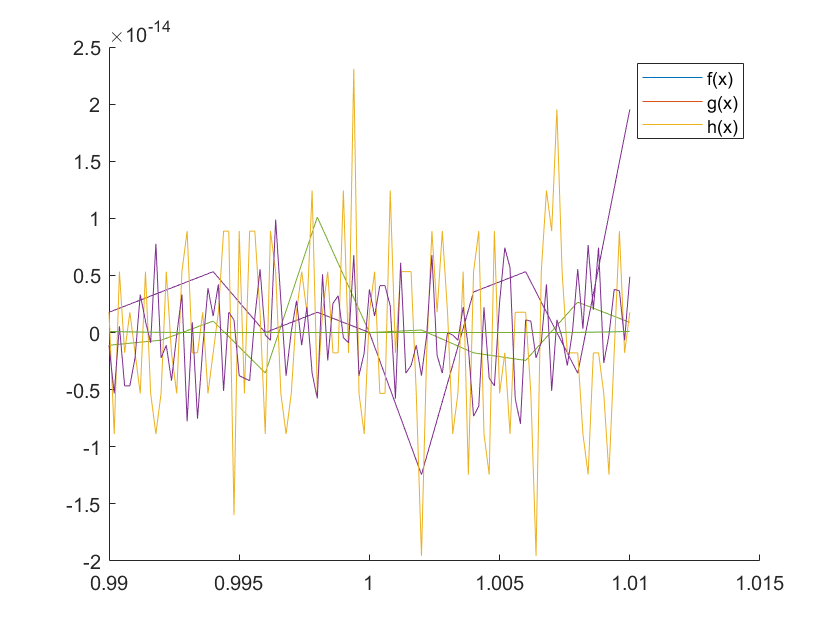
\includegraphics[width=10cm]{Aplot.png}
    \caption{$f(x)$, $g(x)$ and $h(x)$}
    \label{fig:1L}
\end{figure}
\indent Although those three function are "similar", we can see big difference from the chart and the plot. The purple line and the yellow line are obviously unstable and have great vibration. That is because the yellow one has the greatest arithmetic operations and has the most accumulated error while the purple one is next to is.

\section*{Programming 2}

There are 25 numbers in this normalized FPN system.\\
All the numbers are listed as follow: 
0.5 -0.5 0.625 -0.625 0.75 -0.75 0.875 -0.875 1 -1 1.25 -1.25 1.5 -1.5 1.75 -1.75 2 -2 2.5 -2.5 3 -3 3.5 -3.5 0 \\
It verifies the theorem that the cardinal number of this system is:$2^3 \times (1-(-1)+1)+1 = 25$.\\
The plot of the normalized FPN on the real axis:\\
 \begin{figure}[htp]
    \centering
    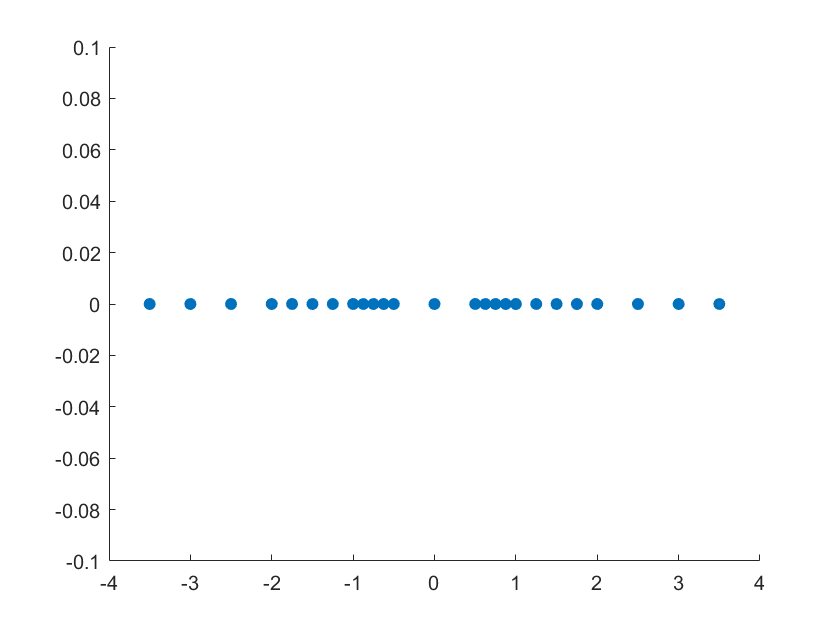
\includegraphics[width=10cm]{Bplot1.png}
    \caption{Normalized FPN}
    \label{fig:1L}
\end{figure}

The plot of the FPN with subnormal one on the real axis:\\
 \begin{figure}[htp]
    \centering
    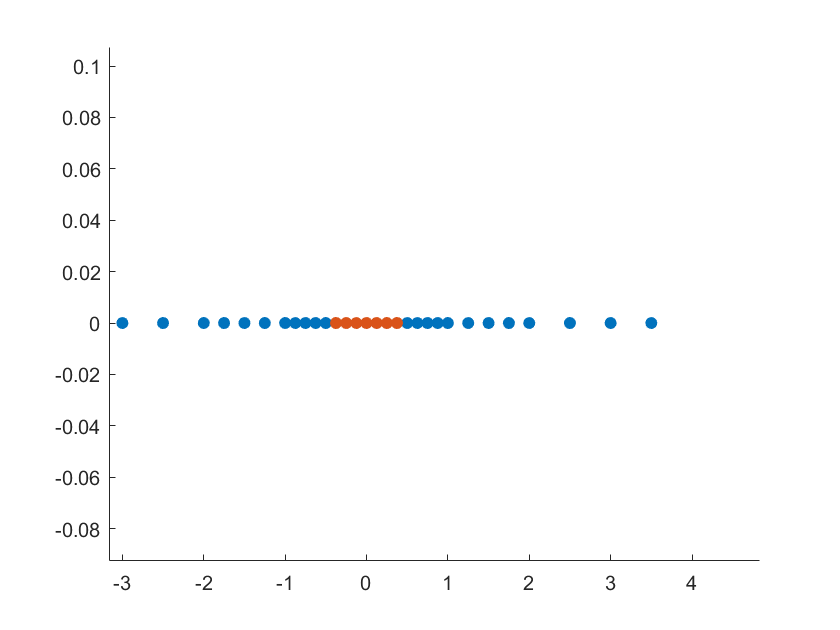
\includegraphics[width=10cm]{Bplot.png}
    \caption{With subnormal FPN}
    \label{fig:1L}
\end{figure}
\end{document} 
